Definicje zostały zaczerpnięte z literatury, z pozycji \cite{Fenner2020}, \cite{Geron2020}, \cite{Seenappa} oraz \cite{vanDerMaaten}.

\newcommand{\mlDefinitionIndex}{1}
\newcommand{\incrementMlDefinitionIndex} {
    \pgfmathtruncatemacro{\mlDefinitionIndex}{\mlDefinitionIndex + 1}
}

\noindent
\textbf{Definicja \mlDefinitionIndex.}
\incrementMlDefinitionIndex
Zbiór treningowy - zbiór danych, który jest używany do trenowania modelu uczenia maszynowego.

\noindent
\textbf{Definicja \mlDefinitionIndex.}
\incrementMlDefinitionIndex
Zbiór walidacjny - zbiór danych, który jest używany do sprawdzenia wydajności modelu uczenia maszynowego.

\noindent
\textbf{Definicja \mlDefinitionIndex.}
\incrementMlDefinitionIndex
Zbiór testowy - zbiór danych używany do oceny wydajności modelu uczenia maszynowego
po przeszkoleniu go na zbiorze treningowym i ocenie na zbiorze walidacyjnym.

\noindent
\textbf{Definicja \mlDefinitionIndex.}
\incrementMlDefinitionIndex
Klasyfikacja to proces polegający na przypisaniu obiektów do wcześniej zdefiniowanych klas na podstawie ich cech.

\noindent
\textbf{Definicja \mlDefinitionIndex.}
\incrementMlDefinitionIndex
Regresja liniowa - metoda, w której model liniowy przewiduje wyniki na podstawie ważonej sumy cech wejściowych oraz stałej,
nazywanej punktem obciążenia lub punktem przecięcia.

\noindent
\textbf{Definicja \mlDefinitionIndex.}
\incrementMlDefinitionIndex
Walidacja krzyżowa to proces, w którym dane dzielone są na kilka części (przyjmujemy k) zwanych "złożeniami"
(lub "foldami" - stąd nazwa k-Fold Cross-Validation). Model jest trenowany na $k-1$ złożeń, a testowany na pozostałym z nich.
Proces ten jest powtarzany $k$ razy, za każdym razem używając innego złożenia do testowania, a pozostałych do treningu.
Jeżeli różnica w wydajności jest znacząca, uzasadniony jest sceptyzm odnośnie pojedynczych wyników pomiaru wydajności systemu.
Z drugiej strony, jeżeli wszystkie wyniki są podobne, można mieć dużą dozę pewności, że niezależnie od konkretnego podziału
na dane testowe i treningowe, wydajność systemu będzie podobna.
Końcowa ocena modelu jest uzyskiwana poprzez uśrednienie wyników z każdej iteracji.

\noindent
\textbf{Definicja \mlDefinitionIndex.}
\incrementMlDefinitionIndex
Warstwa Rescaling mnoży każde wejście przez ustalony współczynnik skalujący.
Zastosowanie tej techniki jest przydatne, gdy różne cechy danych wejściowych mają różne zakresy wartości.
Poprzez jednolite skalowanie, model może efektywniej uczyć się wzorców, a proces optymalizacji staje się stabilniejszy.

\noindent
\textbf{Definicja \mlDefinitionIndex.}
\incrementMlDefinitionIndex
Warstwa Conv2D tworzy jądro splotu, które jest nakładane na dane wejściowe w jednym wymiarze przestrzennym (lub czasowym), 
aby wygenerować tensor danych wyjściowych.
Dodatkowo, jeśli stosowana jest funkcja aktywacji, jest ona stosowana również do danych wyjściowych.

\noindent
\textbf{Definicja \mlDefinitionIndex.}
\incrementMlDefinitionIndex
Warstwa MaxPooling2D dokonuje redukcji wymiarów danych wejściowych wzdłuż ich wymiarów przestrzennych (wysokości i szerokości),
wybierając maksymalną wartość z każdego okna o rozmiarze określonym przez wybrany współczynnik $pool\_size$,
dla każdego kanału danych wejściowych.
Okno to jest przesuwane o określoną liczbę kroków wzdłuż obu wymiarów.

\noindent
\textbf{Definicja \mlDefinitionIndex.}
\incrementMlDefinitionIndex
Warstwa Dropout losowo zeruje jednostki wejściowe z prawdopodobieństwem określonym
przez wybrany współczynnik dropout na każdym etapie treningu, co pomaga unikać przeuczenia modelu.
Jednostki, które nie zostały wyzerowane, są skalowane w górę przez mnożenie przez $\frac{1}{1 - współczynnikDropout}$,
aby suma wartości wejściowych pozostała niezmieniona.

\noindent
\textbf{Definicja \mlDefinitionIndex.}
\incrementMlDefinitionIndex
Bias (błąd obciążenia) to błąd wynikający z niepoprawnych założeń w procesie uczenia maszynowego.
Oznacza różnicę między przewidywaną wartością modelu a rzeczywistą wartością.

\noindent
\textbf{Definicja \mlDefinitionIndex.}
\incrementMlDefinitionIndex
Funkcje aktywacji są nieliniowe, co pozwala na modelowanie złożonych funkcji i wprowadza nieliniowość do sieci.
Równanie matematyczne opisujące działanie sieci neuronowej ma postać: $Y' = g(W_o + X^T * W)$, gdzie:
$Y'$ to przewidywana wartość wyjściowa,
$W_o$ to wartość bias,
$X^T$ to transpozycja macierzy wejściowej $X$,
$W$ to przypisane wagi,
a $g$ to funkcja aktywacji.

\noindent
\textbf{Definicja \mlDefinitionIndex.}
\incrementMlDefinitionIndex
Funkcja ReLU (ang. Recified Linear Unit) - funkcja aktywacji.
Jest ciągła, ale nieróżniczkowalna w punkcie z = 0, a jej pochodna dla z < 0 wynosi 0.
Spisuje się bardzo dobrze w modelowaniu złożonych funkcji, a dodatkowym aututem jest jej szybkość przetwarzania.
Nie ma maksymalnej wartości wyjściowej.

\begin{figure}[ht]
	\centering
	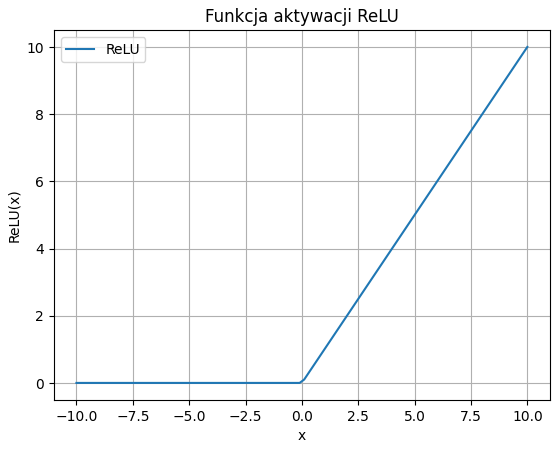
\includegraphics[width=8cm]{resources/machine-learning/images/def_relu.png}
	\caption{Funkcja aktywacji ReLU.
		Źródło: opracowanie własne na podstawie:
        Géron A.: Uczenie maszynowe z użyciem Scikit-Learn i TensorFlow. Helion SA, Gliwice 2020.}
    \label{Fig:def-1}
\end{figure}

\noindent
\textbf{Definicja \mlDefinitionIndex.}
\incrementMlDefinitionIndex
Warstwa Flatten (spłaszczona) ma za zadanie przekształcić każdy obraz wejściowy w tablicę jednowymiarową.
Nie zawiera żadnych parametrów, a jej jedynym celem jest proste, wstępne przetworzenie danych.

\noindent
\textbf{Definicja \mlDefinitionIndex.}
\incrementMlDefinitionIndex
Przeuczenie to sytuacja, w której algorytm dopasowuje się zbyt dokładnie do danych treningowych,
co prowadzi do modelu, który nie potrafi dokładnie prognozować ani wnioskować na podstawie nowych danych spoza zbioru treningowego.

\begin{figure}[ht]
	\centering
	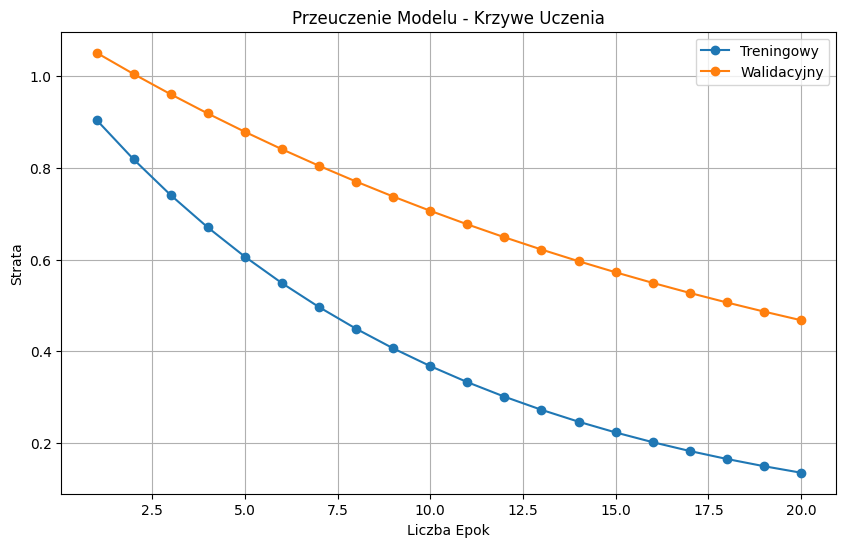
\includegraphics[width=9cm]{resources/machine-learning/images/def_overfit.png}
	\caption{Zobrazowane przeuczenie modelu}
    \label{Fig:def-2}
\end{figure}

\noindent
\textbf{Definicja \mlDefinitionIndex.}
\incrementMlDefinitionIndex
Warstwa Dense (w pełni połączona) zarządza samodzielnie swoją macierzą wag,
zawierającą wszystkie wagi połączeń między neuronami a wejściami do nich, oraz wekorem obciążeń.
Zawiera najczęściej bardzo dużo parametrów, dzięki czemu model uzyskuje swobodę w dopasowaniu do danych treningowych.
Jednocześnie, grozi mu również przez to ryzyko przetrenowania,
zwłaszcza w przypadku korzystania z mniejszych zestawów danych.

\noindent
\textbf{Definicja \mlDefinitionIndex.}
\incrementMlDefinitionIndex
Regularyzacja to technika stosowana w celu zapobiegania przeuczeniu modelu.
Działa poprzez dodanie kary do funkcji kosztu, co penalizuje zbyt złożone modele.

\noindent
\textbf{Definicja \mlDefinitionIndex.}
\incrementMlDefinitionIndex
Regularyzacja L2 służy do ograniczania wag sieci neuronowych,
natomiast regularyzacja L1 przydaje się do tworzenia modeli rzadkich (w których wiele wag ma wartość równą 0). 
Zazwyczaj powinno się stosować ten sam typ regularyzatora we wszystkich wartstwach sieci.

\noindent
\textbf{Definicja \mlDefinitionIndex.}
\incrementMlDefinitionIndex
Epoka to pełny cykl przez cały zbiór danych treningowych, w której model przetwarza wszystie dostępne dane treningowe.
Liczba epok określa ile razy model przejdzie przez cały zbiór danych treningowych.

\noindent
\textbf{Definicja \mlDefinitionIndex.}
\incrementMlDefinitionIndex
Dokładność modelu to stosunek oznaczonych prawidłowo wartości do przykładów sklasyfikowanych nieprawidłowo.

\noindent
\textbf{Definicja \mlDefinitionIndex.}
\incrementMlDefinitionIndex
Koncepcja macierzy pomyłek polega na zliczaniu przypadków zaklasyfikowania próbek z klasy A jako przykładów należących do klasy B.
Aby utworzyć taką macierz, należy uzyskać zbiór prognoz, które porówywane są z rzeczywistymi wartościami docelowymi.

\noindent
\textbf{Definicja \mlDefinitionIndex.}
\incrementMlDefinitionIndex
Strata modelu to wartość, która wskazuje,
jak bardzo prognozy modelu różnią się od rzeczywistych wartości dla pojedynczych przykładów.
Idealnie przewidziane wartości mają stratę równą zeru,
natomiast im większa różnica między prognozami a rzeczywistością, tym wyższa jest strata.

\noindent
\textbf{Definicja \mlDefinitionIndex.}
\incrementMlDefinitionIndex
Algorytm t-SNE (t-Distributed Stochastic Neighbor Embedding) to technika redukcji wymiarowości,
która szczególnie dobrze nadaje się do wizualizacji wielowymiarowych zbiorów danych.
Można ją zaimplementować przy użyciu aproksymacji Barnesa-Huta,
co umożliwia stosowanie jej na dużych, rzeczywistych zbiorach danych.